\section[Desenvolvimento do Projeto]{Desenvolvimento do Projeto}

\subsection{Repositório do Código Fonte do Projeto}

O projeto possui repositórios separados para o backend, frontend e wiki:

\begin{itemize}
  \item \textbf{Backend:} \url{https://tools.ages.pucrs.br/ensportive/ensportive-backend.git}
  \item \textbf{Frontend:} \url{https://tools.ages.pucrs.br/ensportive/ensportive-frontend.git}
  \item \textbf{Wiki:} \url{https://tools.ages.pucrs.br/ensportive/ensportive-wiki.git}
\end{itemize}

\subsection{Banco de Dados Utilizado}

O projeto utiliza o banco de dados \textbf{PostgreSQL}, acessado via \ac{jdbc} através do
Spring Boot. A configuração da \textit{datasource} na aplicação é:

\begin{verbatim}
spring:
  application:
    name: Ensportive
  datasource:
    url: jdbc:postgresql://localhost:5432/ensportive
    username: ensportive
    password: a12345678
  jpa:
    hibernate:
      ddl-auto: update
    show-sql: true
\end{verbatim}

\begin{figure}[H]
    \centering
    \small
    \caption{Modelo de dados ENSportive}
    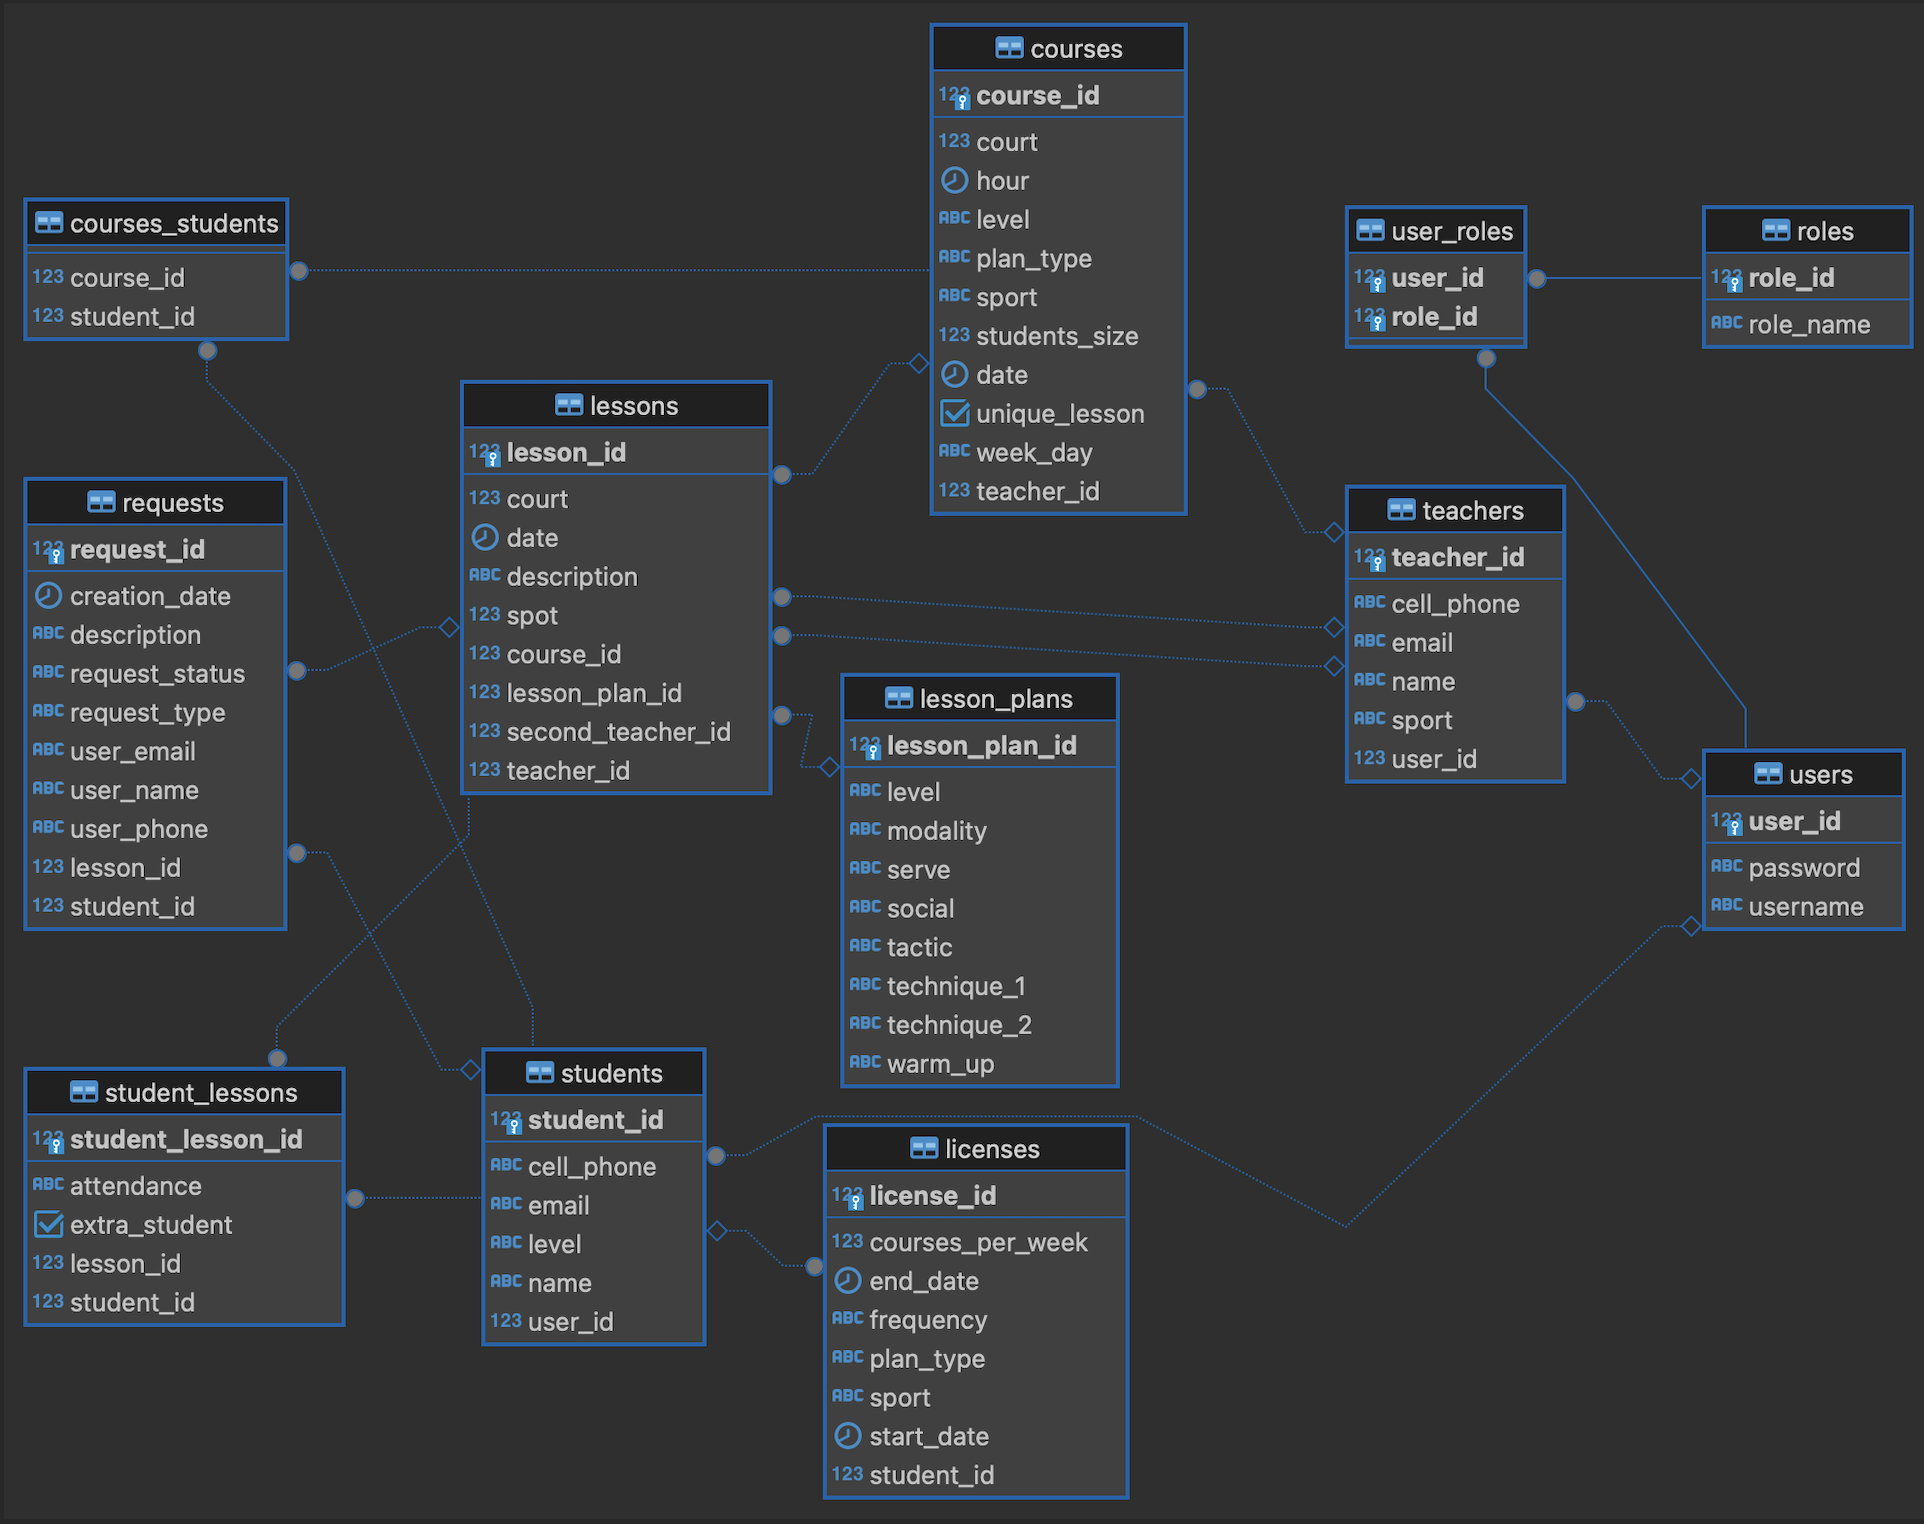
\includegraphics[width=1\linewidth]{conteudo//2 - ages I//conteudo//figures/DadosENSportive.png}
    Fonte: Arquivos pessoais
    \label{fig:dados-ensportive}
\end{figure}

\subsection{Arquitetura Utilizada}

O projeto utiliza uma arquitetura para desenvolvimento web baseada em
\textbf{microsserviços}, com frontend e backend desacoplados, permitindo que
cada parte evolua de forma independente e que futuramente os módulos possam
ser integrados ao ecossistema completo da ENSportive.

\begin{figure}[H]
    \centering
    \small
    \caption{Arquitetura Clean ENSportive}
    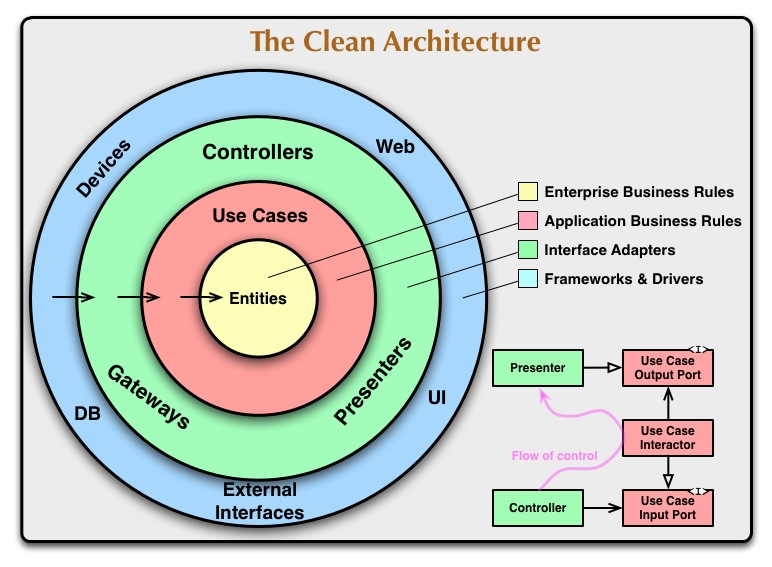
\includegraphics[width=1\linewidth]{conteudo//2 - ages I//conteudo//figures/ArquiteturaENSportive.jpg}
    Fonte: Arquivos pessoais
    \label{fig:arquitetura-ensportive}
\end{figure}

\subsection{Infraestrutura Utilizada}

\begin{figure}[H]
    \centering
    \small
    \caption{Infraestrutura ENSportive}
    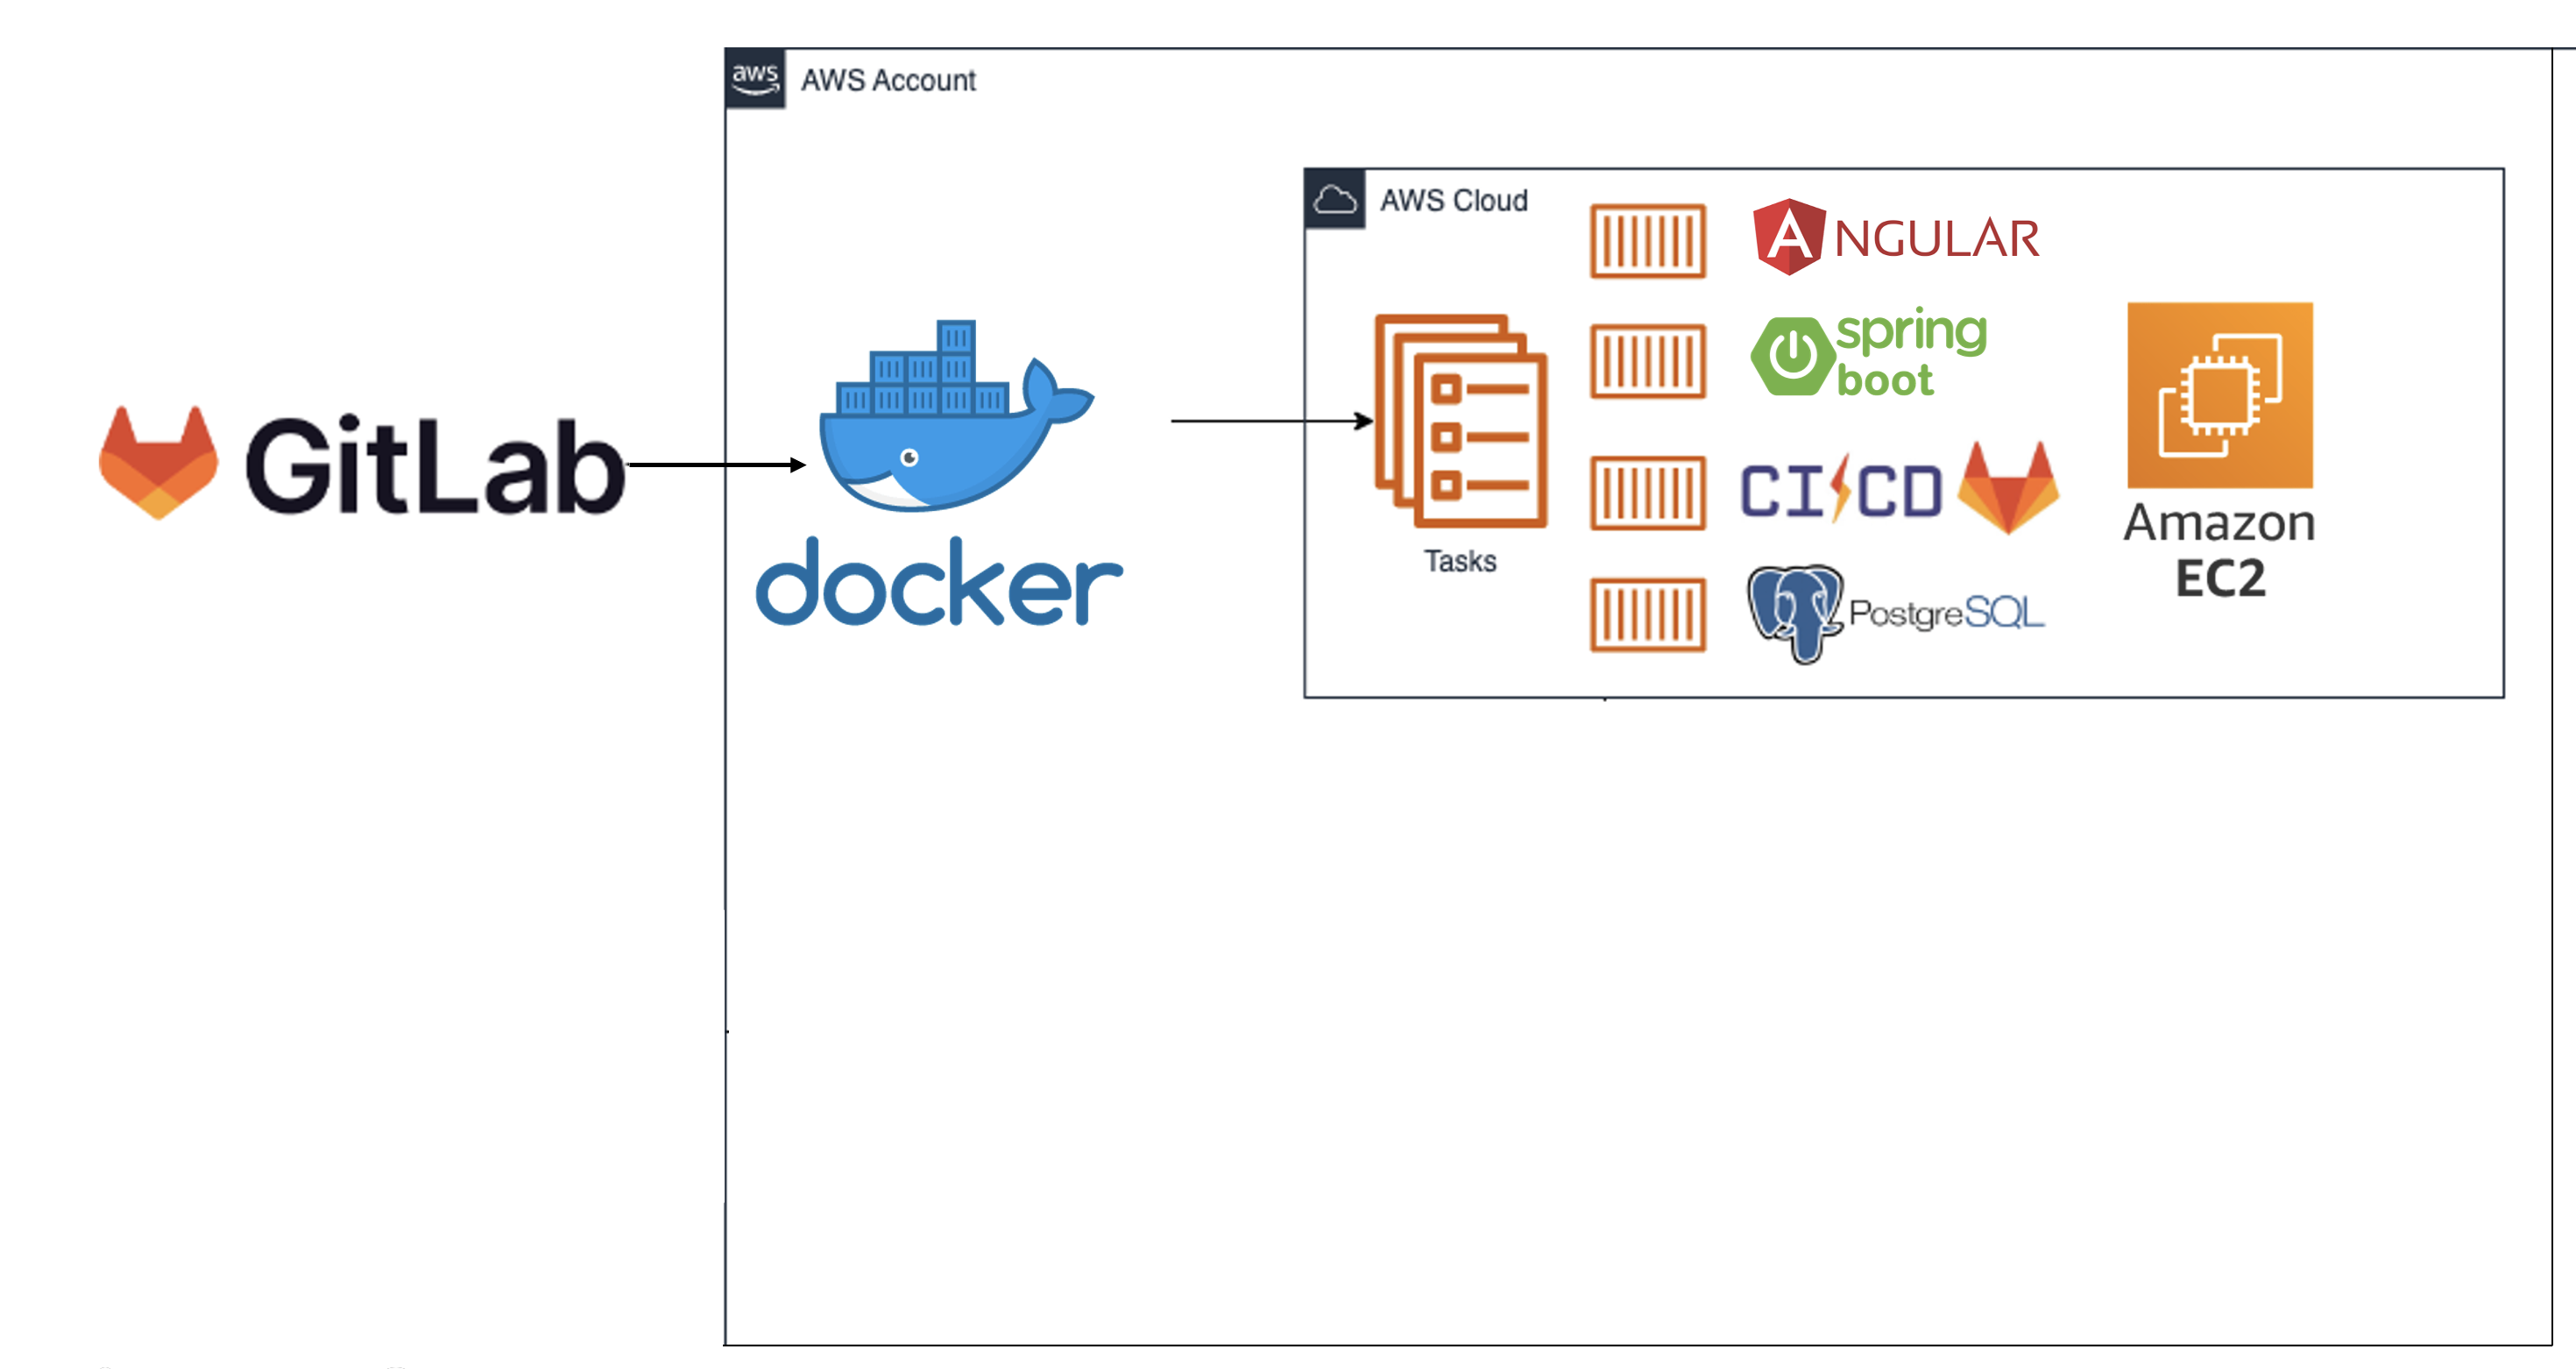
\includegraphics[width=1\linewidth]{conteudo//2 - ages I//conteudo//figures/InfraENSportive.png}
    Fonte: Arquivos pessoais
    \label{fig:infra-ensportive}
\end{figure}

\subsection{Protótipos das Telas Desenvolvidas}

O protótipo foi desenvolvido no Figma e validado pela stakeholder. O fluxo
inicia com uma tela de login que redireciona o usuário conforme seu perfil:
administrador (gestão de alunos, professores e planos), professor (visualização
de horários, edição de plano de aula e feedback) ou aluno (visualização de faltas,
solicitação de reposição, cancelamento de aulas e feedback).

Acesso ao protótipo:
\url{https://www.figma.com/proto/gfr7V9yzPnGPW0tZx3N7Ue/ENSportiveWeb}

\subsection{Tecnologias Utilizadas}

\begin{itemize}
  \item \textbf{Angular 17:} Framework frontend utilizado para o desenvolvimento
    das interfaces da aplicação, escolhido pelo time por trazer recursos modernos
    e diferenciados em relação ao React, tecnologia mais comum entre os alunos da \ac{ages}.

  \item \textbf{Bootstrap 5:} Biblioteca de componentes \ac{css} utilizada para padronização
    visual das telas, garantindo responsividade e consistência no design.

  \item \textbf{Java Spring Boot:} Framework backend responsável pela lógica de negócio
    e exposição das APIs \ac{rest}, com gerenciamento de dependências via Maven.

  \item \textbf{Docker:} Utilizado para containerização dos serviços, facilitando o
    ambiente de desenvolvimento e a futura implantação em produção.

  \item \textbf{Maven:} Ferramenta de gerenciamento de dependências e build do projeto
    backend.

  \item \textbf{PostgreSQL:} Banco de dados relacional utilizado para persistência
    dos dados da aplicação.
\end{itemize}
